\documentclass{article}
\usepackage[spanish]{babel}
\usepackage[onehalfspacing]{setspace}
\usepackage[utf8]{inputenc}
\usepackage{amsmath}
\usepackage{amssymb}
\usepackage{verbatim}
\usepackage{graphicx}
\usepackage{listings}
\usepackage{fullpage}
\usepackage{color}
\usepackage{fancyvrb}
\usepackage{hyperref}
\hypersetup{%
	pdfborder = {0 0 0}
}

\definecolor{mygreen}{rgb}{0,0.6,0}
\definecolor{mygray}{rgb}{0.5,0.5,0.5}
\definecolor{mymauve}{rgb}{0.58,0,0.82}

\lstset{ %
	backgroundcolor=\color{white},   % choose the background color; you must add \usepackage{color} or \usepackage{xcolor}
	basicstyle=\footnotesize,        % the size of the fonts that are used for the code
	breakatwhitespace=false,         % sets if automatic breaks should only happen at whitespace
	breaklines=true,                 % sets automatic line breaking
	captionpos=b,                    % sets the caption-position to bottom
	commentstyle=\color{mygreen},    % comment style
	frame=single,                    % adds a frame around the code
	keepspaces=true,                 % keeps spaces in text, useful for keeping indentation of code (possibly needs columns=flexible)
	numbers=left,                    % where to put the line-numbers; possible values are (none, left, right)
	numbersep=5pt,                   % how far the line-numbers are from the code
	numberstyle=\tiny\color{mygray}, % the style that is used for the line-numbers
	rulecolor=\color{black},         % if not set, the frame-color may be changed on line-breaks within not-black text (e.g. comments (green here))
	showspaces=false,                % show spaces everywhere adding particular underscores; it overrides 'showstringspaces'
	showstringspaces=false,          % underline spaces within strings only
	showtabs=false,                  % show tabs within strings adding particular underscores
	stepnumber=1,                    % the step between two line-numbers. If it's 1, each line will be numbered
	stringstyle=\color{mymauve},     % string literal style
	tabsize=4,
	title=\lstname                   % show the filename of files included with \lstinputlisting; also try caption instead of title
}


\author{José Luis Cánovas Sánchez}
\title{ARQUITECTURAS DE REDES AVANZADAS\\QUAGGA}
\date{}
\begin{document}
\maketitle

\begin{center}
	
\includegraphics[scale=0.3]{images/mascota.png}
\end{center}

\begin{abstract}
	En este informe se redacta el desarrollo usando la herramienta QUAGGA para el despliegue del escenario de red IPv6.
	%TODO: terminar
\end{abstract}

\tableofcontents

\section{Introducción}

Quagga es un proyecto de software que provee de utilidades para encaminamiento de red en sistemas UNIX, proveyendo el demonio zebra originario de otro proyecto y que permite aplicar configuraciones de algoritmos de encaminamiento a las tablas de red de la máquina. Los algoritmos se ejecutan como demonios que toman la información de la red y aplican protocolos conocidos, tales como OSPF, RIP, IS-IS y BGP, en múltiples de sus versiones, y por medio de zebra los aplican a la red.

\begin{center}
	\begin{BVerbatim}
+----+  +----+  +-----+  +-----+
|bgpd|  |ripd|  |ospfd|  |zebra|
+----+  +----+  +-----+  +-----+
|
+---------------------------|--+
|                           v  |
|  UNIX Kernel  routing table  |
|                              |
+------------------------------+

    Quagga System Architecture
	\end{BVerbatim}
\end{center}

Vamos a configurar tres de estos protocolos con Quagga en cuatro máquinas que harán las veces de routers. %TODO: comprobar número de sección
En la sección 2 se muestra la topología que se va a implementar. En las secciones 3 a 6 se explicará cómo instalar y configurar Quagga con los mecanismos OSPF, RIP y BGP para IPv6.

La topología usada en este estudio de Quagga se asemeja mucho a la de la práctica 1 de ARA, pero se puede llevar a otros proyectos, como LEGO, fácilmente. Más adelante se muestra la topología en \autoref{fig:topology}, y con hacer corresponder R1 y R2 con los routers de las organizaciones de LEGO, las redes XXXX:0:1::/64 con las subredes de cada organización, y las subredes XXXX::/64 con una subred un nivel más interna, tenemos la topología de LEGO ampliada. La salida a internet se debería realizar con tunelado a IPv4 en R1 y R2, si no se dispone de IPv6 pública. En caso de tener un rango de direcciones IPv6 públicas, habría que cambiar los valores de cada subred para que sean válidos, pero queda fuera de este estudio.

\section{Topología de trabajo}


Partimos de dos Sistemas Autónomos con números 17 y 71 (curiosidad, son primos \hyperref{https://en.wikipedia.org/wiki/Permutable_prime}{}{}{\underline{permutables}}  entre sí) y mecanismo de encaminamiento interno por OSPF, con un área backbone y un área 1 stub para el AS17, un mecanismo basado en RIPng para el AS1 y BGP entre ambos AS, como se muestra en la \autoref{fig:topology}.


\begin{figure}[!h]
	\centering
	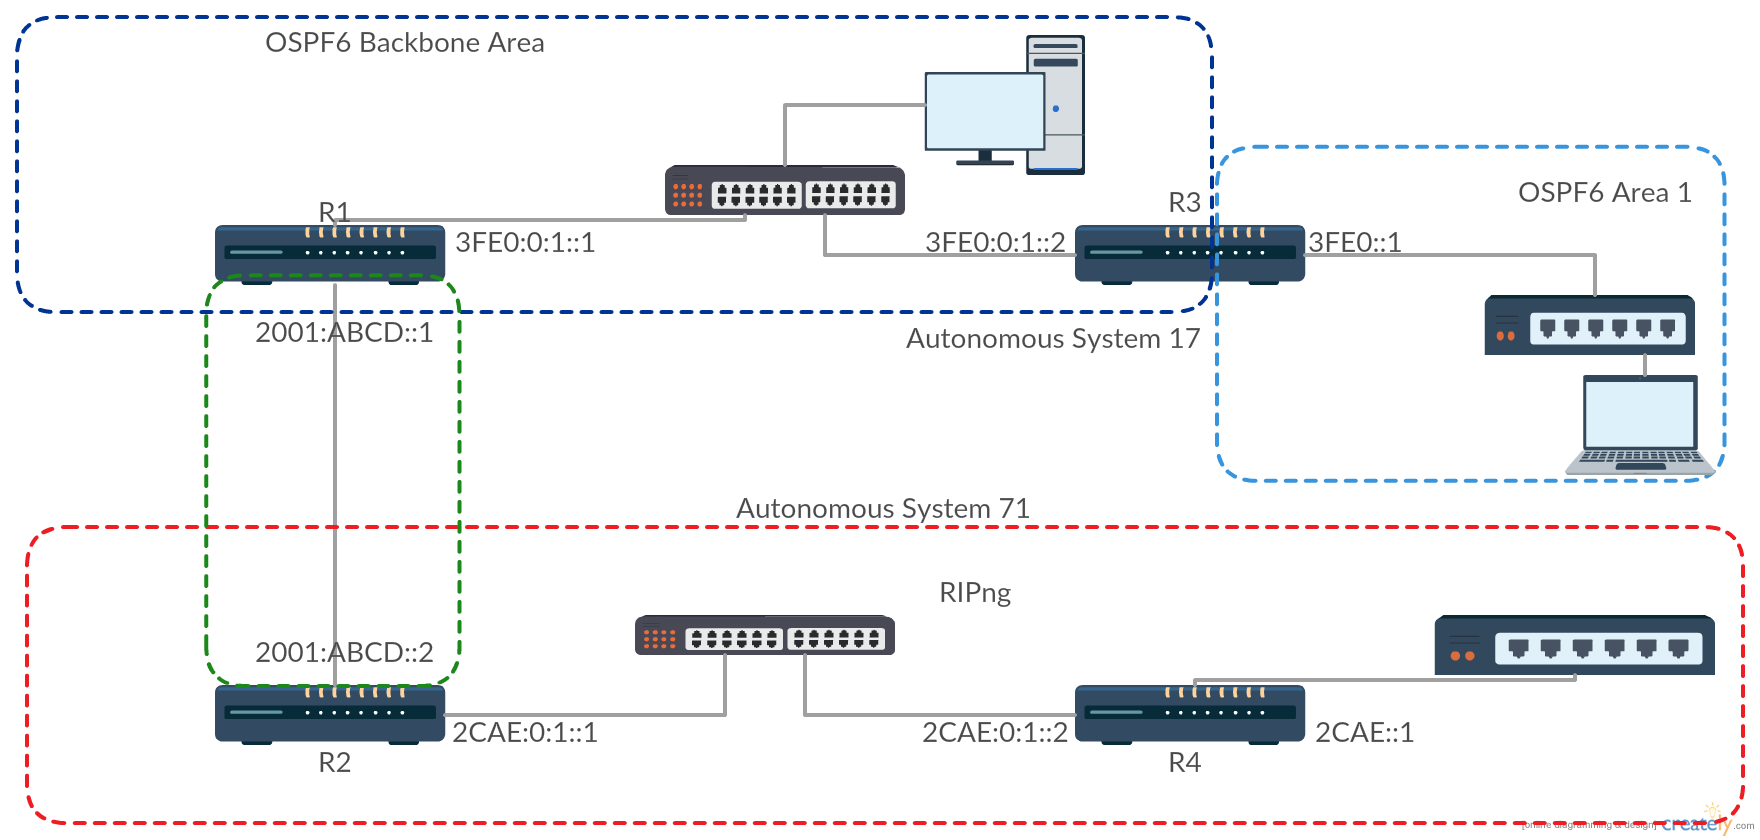
\includegraphics[scale=0.29]{images/Topology.png}
	\caption{Topología}
	\label{fig:topology}
\end{figure}


\section{Instalar Quagga}
%TODO: más configuración mínima de interfaces
%interface FastEthernet1/0
%no ip address
%duplex half
%ipv6 address 3FE0:0:1::/64 eui-64
%ipv6 enable
%ipv6 ospf 100 area 0

\section{Configuración de OSPF}
%ipv6 router ospf 100
%router-id 1.1.1.1
%log-adjacency-changes
%redistribute bgp 10


\section{Configuración de RIPng}

\section{Configuración de BGP}
% http://www.cisco.com/c/en/us/td/docs/ios/12_2/ip/configuration/guide/fipr_c/1cfbgp.html#wp1001080

%
%!
%router bgp 13
%bgp router-id 1.1.1.1
%no bgp default ipv4-unicast
%!--- Without configuring ""no bgp default ipv4-unicast"" only IPv4 will be !--- advertised
%bgp log-neighbor-changes
%neighbor 2001:ABCD::2 remote-as 50
%!
%address-family ipv6
%neighbor 2001:ABCD::2 activate
%network 3FE0:0:1::/64
%network 3FE0::/64
%exit-address-family
%!


\end{document}
